\documentclass[12pt]{beamer}
\setbeamertemplate{navigation symbols}{}

\usepackage{graphicx}
\usepackage{hyperref}
\graphicspath{ {images/} }

\title{Icaramba!\\ Iphone vulnerabilities compromise personal data}
\titlegraphic{ 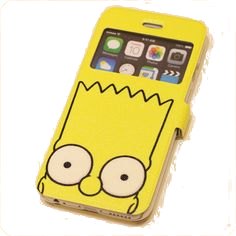
\includegraphics[width=6em]{bart_phone_case.png} }
\author{Innovatech}
\date{September 13, 2016}

\begin{document}

\begin{frame}
	\titlepage
\end{frame}

\section{Table of Contents}
\begin{frame}
	\frametitle{Table of contents}
	\tableofcontents[]
\end{frame}

\section{Initial Attack}
\begin{frame}
	\frametitle{An innocuous text}
	\begin{center}
		\begin{quote}
			New secrets about torture of Emiratis in state prisons \url{http://go.osu.edu/not_a_virus}
		\end{quote}
	\end{center}
\end{frame}
\note{An innocuous text was sent to a human rights activist from UAE. Inside there was a link that would remotely jailbreak his Iphone.\\ Since he had already been targeted before, he notified the security firm 'Citizen Lab'}

\section{How it worked}
\begin{frame}
	\frametitle{What was vulnerable?}
	\begin{center}
		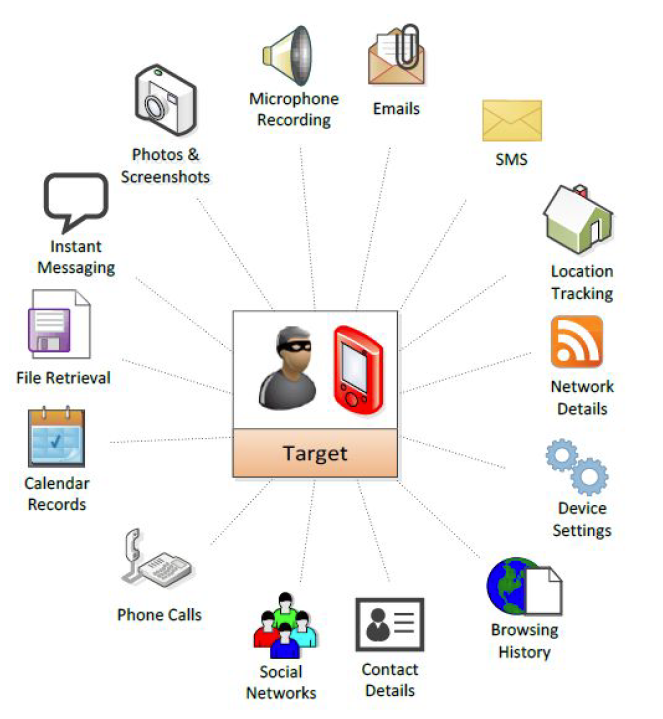
\includegraphics[height=.85\textheight]{vulnerable_data.png}
	\end{center}
\end{frame}
\note{The software was evaluated and it was determined that this link would've given access to all data accessible by the phone. It in fact incorporated three unknown vulnerabilities (also known as zero days)}

\section{Who did it?}
\begin{frame}
	\frametitle{Who did it?}
\end{frame}

\begin{frame}
	\frametitle{References}
	\textbf{Images}
	\begin{itemize}
		\item Bart Iphone case-Pinterest
		\item Diagram of vulnerable data-Motherboard(https://motherboard.vice.com/read/government-hackers-iphone-hacking-jailbreak-nso-group)
	\end{itemize}
	\textbf{Information}
	\begin{itemize}
		\item Motherboard, \href{https://motherboard.vice.com/read/government-hackers-iphone-hacking-jailbreak-nso-group}{Government Hackers Caught Using Unprecedented iPhone Spy Tool}
	\end{itemize}
\end{frame}

\end{document}
